\documentclass[a4paper,12pt]{report}
\usepackage[utf8]{inputenc} % Kodierung
\usepackage[ngerman]{babel} % Sprache
\usepackage{geometry} % to change the page dimensions
\geometry{left=2.5cm, right=2cm, top=3cm, bottom=3cm} % or letterpaper (US) or a5paper or....
% \geometry{margin=2in} % for example, change the margins to 2 inches all round
% \geometry{landscape} % set up the page for landscape
%   read geometry.pdf for detailed page layout information
\usepackage{graphicx}
\usepackage{float}
\usepackage{fancyhdr}
\usepackage[bottom,hang]{footmisc}
\usepackage{tabularx}
\usepackage{setspace} % Paket für Zeilenabstand
\usepackage{acronym} % Paket für Abkürzungsverzeichnis
\usepackage[numbers,square]{natbib} % numbers ist notwendig für alphadin, squar sorgt für eckige Klammern

%\setlength{\textwidth}{14cm}
%\setlength{\textheight}{25.5cm}
%\setlength{\topmargin}{-2.0cm}
%\setlength{\oddsidemargin}{0cm}
%\setlength{\evensidemargin}{0cm}

\fancypagestyle{plain}{
\fancyhead{}
\renewcommand{\headrulewidth}{0.0pt}}

\pagestyle{fancy}
\renewcommand{\chaptermark}[1]{\markboth{#1}{}}
\fancyhf{}
\fancyhead[R]{}
\fancyhead[L]{\textbf{\nouppercase\leftmark}}
\fancyfoot[R]{\thepage}
\fancyfoot[L]{}
\renewcommand{\headrulewidth}{0.5pt}

% 1.5 facher Zeilenabstand
\onehalfspacing
% weniger Silbentrennung aber dafür mehr Wortzwischenräume
\sloppy

\begin{document}

%===================================================================== Titlepage
\begin{titlepage}
\centering
\vfill
{\bfseries\Huge Masterarbeit}\\[2cm]
{\bfseries\Large Modellierung der Qualitätsmanagementprozesse}\\[0.2cm]
{\bfseries\Large für die Marktüberwachung und Vigilanz in der}\\[0.2cm]
{\bfseries\Large Entwicklung von Medizinprodukten unter}\\[0.2cm]
{\bfseries\Large Berücksichtigung der MDR EU 2017/745}\\
\vfill
vorgelegt von
\vfill
{\large Jens Noack}\\
\vfill
in Kooperation mit der\\[1cm]
{\large W.O.M. WORLD OF MEDICINE GmbH}\\[1cm]
\begin{center}
\begin{minipage}[c]{0.3\textwidth}
   \includegraphics[width  = 3cm]{Images/wom_logo}
  \end{minipage}
\begin{minipage}[c]{0.2\textwidth}
   \includegraphics[width  = 3cm]{Images/akad_logo}
  \end{minipage}
\end{center}
\vfill
\begin{center}\parbox{0cm}{\begin{tabbing}
xxxxxxxxxx \= xxxxxxxx \kill
Hochschule:\quad\quad\quad\quad\quad\quad\quad\quad\quad \= AKAD Bildungsgesellschaft \\
Studiengang: \> Wirtschaftsingenieurwesen \\
\> Master of Engineering \\
Matrikelnummer: \> 2929271 \\
Erstgutachter: \> Dr. Andrea Herrmann\\
Betreuer Firma: \> Dr. Jan Bischof
\end{tabbing}}
\end{center}
\end{titlepage}

%===================================================================== Kurzfassung
\addcontentsline{toc}{chapter}{Kurzfassung} %sorgt für eintrag ins inhaltsverzeichnis
\chapter*{Kurzfassung} %  *-> erstellt unnummeriertes chapter

Kurzfassung Inhalt äöü ÄÖÜ \cite[S. 15]{Freund2014}

%===================================================================== Verzeichnisse
\tableofcontents %Inhaltsverzeichnis
\listoffigures %Abbildungsverzeichnis
\listoftables %Tabellenverzeichnis
\chapter*{Abkürzungsverzeichnis} %  *-> erstellt unnummeriertes chapter
\begin{acronym}[XXXXX] %Option in eckigen Klammern ist längste Abkürzung
 \acro{BPM}{Business Process Management}
 \acro{BPMN}{Business Process Model and Notation}
 \acro{EPK}{Ereignisgesteuerte Prozesskette}
 \acro{PMS}{Post Market Surveillance}
 \acro{UML}{Unified Modeling Language}
\end{acronym}

%===================================================================== Einleitung
\chapter{Einleitung}\label{chap:Einleitung}

%===================================================================== Cahpter 2
\chapter{Grundlagen}\label{chap:Grundlagen}
In diesem Kapitel werden wichtige Grundlagen für das Verständnis der Zusammenhänge und die Einordnung der Bedeutung der folgenden Kapitel vermittelt. Dazu wird zunächst das Themenfeld der Geschäftsprozessmodellierung grob beleuchtet, wobei mit BPMN 2.0 eine Modellierungstechnik vorgestellt wird, die für die Visualisierung und Modellierung von Geschäftsprozessen im Rahmen dieser Arbeit verwendet wird. Anschließend wird der regulatorische Rahmen auf dem Medizinproduktemarkt sowie die dort vorherrschenden Anforderungen an die Qualitätsprozesse nach der Markteinführung vorgestellt.

\section{Analyse, Visualisierung und Modellierung von Geschäftsprozessen}\label{sec:BPM}
Dieses Kapitel beinhaltet einen groben Überblick über die Grundlagen für das Management von Geschäftsprozessen. Es stellt somit in gewisser Weise das ``Handwerkszeug'' für die gestellte Aufgabe dar, da die Analyse und Anpassung von Geschäftsprozessen einen essentiellen Anteil am Hauptziel dieser Arbeit einnimmt.
\subsection{Business Process Management}\label{subsec:BPManagement}
Im rein betriebswirtschaftlichen Sinne bezeichnet \ac{BPM} die Implementierung einer Managementphilosophie, die Unternehmensprozesse als zentralen Erfolgsfaktor eines Unternehmens betrachtet. In Zeiten von Globalisierung, Digitalisierung und dem damit verbundenen permanent ansteigenden Konkurrenzdruck konzentrieren sich Firmen immer mehr auf ihre eigenen Stärken und nutzen das Geschäftsprozessmanagement zur prozessorientierten Gestaltung der Unternehmensstrukturen. Zu den Hauptaufgaben des \ac{BPM} gehören neben dem Dokumentieren auch das Gestalten und Verbessern von Geschäftsprozessen. Dabei wird im Allgemeinen auf standardisierte Modellierungssprachen zurückgegriffen (z.B. UML, EPK oder BPMN), weswegen die IT-Unterstützung für \ac{BPM} eine große Rolle spielt \citep[vgl.][S. 1ff.]{Becker2009}. 

Mit Hilfe von \ac{BPM} ist es Unternehmen möglich ihre Prozesse zu optimieren, so dass diese weniger kosten und schneller werden, wobei trotzdem die Genauigkeit gesteigert wird. Gut angepasste und ``schlanke'' Prozesse sind zudem flexibler und erlauben schneller auf den Markt zu reagieren. Das Ergebnis sind geringere Kosten und eine höhere Kundenzufriedenheit und somit eine bessere allgemeine Performance des Unternehmens. Der Erfolg und die Nachhaltigkeit dieses Konzeptes wird durch die konsequente Einführung von Metriken zur Bestimmung der Leistungsfähigkeit der Prozesse untermauert. Dies ermöglicht schnelle Anpassungen auf neue Situationen, was bei der heutigen Marktdynamik nahezu überlebenswichtig ist \citep[vgl.][S. 7]{Brocke2014}.

Eines der wichtigsten Grundprinzipien von \ac{BPM} ist die permanente Überwachung und Anpassung der Prozesse \citep[S. 11f.]{Brocke2014}. Wie in Abbildung \ref{process_management_cycle} ersichtlich ist, kann das Standardvorgehen bei \ac{BPM} durch einen geschlossenen Zyklus dargestellt werden, in dessen Verlauf ein Prozess ständig analysiert und auf Abweichungen von den Zielen überprüft wird, um entsprechende Änderungen einzuleiten.
\begin{figure}[ht]
\centering
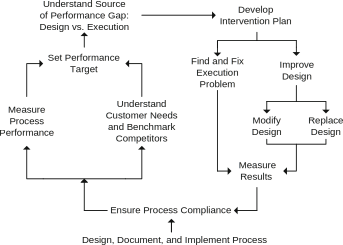
\includegraphics[width=0.7\textwidth]{Images/process_management_cycle}
\caption[Essentieller Zyklus der Geschäftsprozessmodellierung]{Essentieller Zyklus der Geschäftsprozessmodellierung \citep[S. 5]{Brocke2014}}
\label{process_management_cycle}
\end{figure}
\subsection{Business Process Mapping}\label{subsec:BPMapping}

\subsection{Business Process Modeling}\label{subsec:BPModeling}
\subsection{BPMN 2.0}\label{subsec:BPMN}

\section{Regulatorische Anforderungen für Medizingeräte}\label{sec:RegRequ}

\subsection{Gründe und Bedeutung der Regulierung für Medizinprodukte}\label{subsec:Gruende}
\subsection{Überblick über die wichtigsten Normen}\label{subsec:UeberblickNormen}
\subsection{Auswirkungen auf die Entwicklung und den Produktlebenszyklus}\label{subsec:AuswirkungenAufEntwicklung}
\subsubsection{Requirements Engineering}
\subsubsection{Product Lifecycle Management}

\section{Qualitätsprozesse nach Markteinführung medizinischer Geräte}\label{sec:PMProzesse}
\subsection{Vigilance System}\label{subsec:Vigilance}
\subsection{Post Market Surveillance}\label{subsec:PMS}
\subsection{Post Market Clinical Follow-Ups}\label{subsec:PMCF}
\subsection{Integration in die Entwicklungsprozesse}\label{subsec:IntegrationInDevProzesse}

%===================================================================== Chapter 3
\chapter{Aufnahme des Status Quo}\label{chap:AufnahmeStatusQuo}

%===================================================================== Cahpter 4
\chapter{Anpassung des Prozesses unter Berücksichtigung der Medizinprodukteverordnung (MDR) EU 2017/745}\label{chap:AnpassungAnMDR}

%===================================================================== Chapter 5
\chapter{Integration und Umsetzung des neu modellierten Prozesses}\label{chap:Integration}

%===================================================================== Zusammenfassung
\chapter{Zusammenfassung}\label{chap:Zusammenfassung}

%===================================================================== Diskussion
\chapter{Diskussion}\label{chap:Diskussion}

%===================================================================== Vorlagen
%\chapter{}\label{chap:}
%\section{}\label{sec:}
%\subsection{}\label{subsec:}
%\subsubsection{Requirements Engineering}  -- besitzt keine Nummerierung und taucht nicht im toc auf
%\cite[S. X]{<reference>}
%\ac{<Abkürzung>}

%===================================================================== Literaturverz.
\bibliography{literatur}
\bibliographystyle{alphadin}
%\bibliographystyle{abbrv}
% Übersicht unter: https://de.wikibooks.org/wiki/LaTeX-W%C3%B6rterbuch:_bibliographystyle

%===================================================================== Anhang
\appendix
\chapter[Anhang]{}
\newpage
\section{Anhang 1}

%===================================================================== Eidessattl. Vers.
\chapter*{Eidesstattliche Versicherung} %  *-> erstellt unnummeriertes chapter
Ich versichere, dass ich vorliegende Arbeit selbstständig verfasst, keine anderen als die angegebenen Quellen und Hilfsmittel benutzt sowie alle wörtlich oder sinngemäß übernommenen Stellen in der Arbeit gekennzeichnet habe.
\\[2cm]
\noindent\rule{0.35\textwidth}{0.3pt}\rule{0.2\textwidth}{0pt}\rule{0.45\textwidth}{0.3pt}
\\Ort, Datum\rule{0.418\textwidth}{0pt}Unterschrift
\end{document}